\documentclass{article}
\usepackage[utf8]{inputenc}
\usepackage[spanish]{babel}
\usepackage{listings}
\usepackage{subfigure}
\usepackage{graphicx}
\usepackage{url}
\usepackage{multirow}
\usepackage{color}
\usepackage{booktabs}

\setlength{\parindent}{0pt}
\setlength{\parskip}{1em}
\usepackage[margin=3cm,twoside]{geometry} 

\definecolor{mygreen}{rgb}{0,0.6,0}
\definecolor{mygray}{rgb}{0.5,0.5,0.5}
\definecolor{mymauve}{rgb}{0.58,0,0.82}
\lstset{ 
  backgroundcolor=\color{white},   % choose the background color; you must add \usepackage{color} or \usepackage{xcolor}; should come as last argument
  basicstyle=\footnotesize,        % the size of the fonts that are used for the code
  breakatwhitespace=false,         % sets if automatic breaks should only happen at whitespace
  breaklines=true,                 % sets automatic line breaking
  captionpos=b,                    % sets the caption-position to bottom
  commentstyle=\color{mygreen},    % comment style
  deletekeywords={...},            % if you want to delete keywords from the given language
  escapeinside={\%}{)},          % if you want to add LaTeX within your code
  extendedchars=true,              % lets you use non-ASCII characters; for 8-bits encodings only, does not work with UTF-8
  firstnumber=1,                % start line enumeration with line 1000
  frame=single,	                   % adds a frame around the code
  keepspaces=true,                 % keeps spaces in text, useful for keeping indentation of code (possibly needs columns=flexible)
  keywordstyle=\color{blue},       % keyword style
  language=Octave,                 % the language of the code
  morekeywords={*,...},            % if you want to add more keywords to the set
  numbers=left,                    % where to put the line-numbers; possible values are (none, left, right)
  numbersep=5pt,                   % how far the line-numbers are from the code
  numberstyle=\tiny\color{mygray}, % the style that is used for the line-numbers
  rulecolor=\color{black},         % if not set, the frame-color may be changed on line-breaks within not-black text (e.g. comments (green here))
  showspaces=false,                % show spaces everywhere adding particular underscores; it overrides 'showstringspaces'
  showstringspaces=false,          % underline spaces within strings only
  showtabs=false,                  % show tabs within strings adding particular underscores
  stepnumber=1,                    % the step between two line-numbers. If it's 1, each line will be numbered
  stringstyle=\color{mymauve},     % string literal style
  tabsize=2,	                   % sets default tabsize to 2 spaces
  title=\lstname                  % show the filename of files included with \lstinputlisting; also try caption instead of title
}

\title{Tarea No.3: Rectificada}
\author{Dayli Machado (5275)}
\date{\today}

\begin{document}

\maketitle



\section{Grafos y algoritmos empleados}

Para la realización de esta tarea se crearon nuevos grafos pues con los que se contaba de tareas anteriores no se podía realizar la medición del experimeinto y obtener valores medibles pues el número máximo de nodos con los que se contaba era de cinco en todos los grafos.
A continuación se muestran las líneas de código que fueron empleadas para generar los grafos con los que se trabajó durante la medición de los algoritmos seleccionados.

%\newpage
\lstinputlisting[language=Python, firstline=9, lastline=58]{codigomadre.py}

Se generaron cinco grafos: dirigidos y no dirigidos, ponderados, con la cantidad de nodos y arcos aleatorias, así como otro grupo de cinco grafos con una cantidad de nodos y arcos menor para algoritmos que así lo requerían.

Para la selección del tipo de algoritmo se tuvo en cuenta que combinaran con los grafos generados y permitieran obtener valores medibles de ejecución en cada uno. Fueron probados todos y de ellos los que mejores resultados de medición arrojaron fueron los siguientes:

\begin{itemize}
\item Centralidad de intermediación (en lo adelante BC según sus siglas en inglés \textit{Betweenness centrality})
\item \textit{Max clique }(en lo adelante MC)
\item \textit{Greedy} color (en lo adelante GC)
\item Flujo Máximo (en lo adelante MF, por sus siglas en inglés \textit{Maximum flow})
\item Árbol de expansión mínima (en lo adelante MS, por sus siglas en inglés Minimum spanning tree)
\end{itemize}

\subsection{Breve descripción de los algoritmos medidos y su código} 

El algoritmo BC nos brinda la medida de centralidad de un grafo basado en la trayectoria más corta, este devuelve un diccionario de nodos con la medidad de centralidad \cite{bc}.
La centralidad de la interrelación de un nodo es la suma de la fracción de las rutas más cortas de todos los pares que pasan por él \cite{bccentralidad}. Puede usarse en grafos dirigidos y no dirigidos.

El algoritmo MC devuelve el subgrafo más grande que encuentre, se recomienda su uso en grafos no dirigidos, es uno de los algoritmos que más tiempo demora en su ejecución.  

Por su parte el algoritmo GC, lo que hace es colorear un nodo usando diferentes estrategias de coloración que se le pasan como un parámetro dentro de una función.  Devuelve un diccionario con claves que representan nodos y valores que representan la coloración correspondiente \cite{gredy}. Puede emplearse en grafos dirigidos y no dirigidos.

El algoritmo MF determina la ruta a través de la cual puede pasar el máximo flujo, de ahí que uno de los parámetros que requiere es la capacidad, y un su defecto la asume como infinita \cite{mf}. Se recomienda emplearlo en grafos dirigidos.

El algoritmo MS tree devuelve la conexión entre los nodos de modo que la unión entre ellos es un árbol no dirigido ponderado cuya suma de pesos de cada arco es la menor posible \cite{min}.

A continuación se muestra el fragmento de código desarrollado para la medición del tiempo por cada algoritmo:

\lstinputlisting[language=Python, firstline=60, lastline=169]{codigomadre.py}
%\lstinputlisting[language=Python, firstline=267, lastline=278]{codigomadre.py}
\newpage
\section{Resultados} 

Se realizó la medición de los tiempos de los algoritmos teniendo en cuenta la media y la desviación estándar en cada caso. 

Para obtener la cantidad de nodos y arístas de cada grafo empleado se desarrolló el siguiente código:


\lstinputlisting[language=Python, firstline=171, lastline=208]{codigomadre.py}

Para leer de los archivos .csv los valores de media y desviación estándar se usó el siguiente código:


\lstinputlisting[language=Python, firstline=210, lastline=265]{codigomadre.py}

Luego se realizaron los histogramas que reflejan la variación del valor de la media por algoritmo empleado. Seguidamente se muestra un fragmento del códico y los histogramas por algoritmos se muestran en la figura \ref{fig:Fig01} de la página \pageref{fig:Fig01}. En la gráfica se observa que en la mayoría de los algoritmos existe tendencia a ubicarse hacia los valores extremos, excepto en el algoritmo GC, que se aprecia una cantidad de valores igual en cada barra.


\lstinputlisting[language=Python, firstline=8, lastline=37]{Histogramas.py}


\begin{figure}[htbp]

\subfigure[\textit{BC}]{\includegraphics[scale=0.5]{Imagenes/Histograma1.eps}}
\subfigure[\textit{MC}]{\includegraphics[scale=0.5]{Imagenes/Histograma2.eps}}
\subfigure[\textit{GC}]{\includegraphics[scale=0.5]{Imagenes/Histograma3.eps}}
\subfigure[\textit{MF}]{\includegraphics[scale=0.5]{Imagenes/Histograma4.eps}}
\subfigure[\textit{MS} ]{\includegraphics[scale=0.5]{Imagenes/Histograma5.eps}}
\caption{Histograma de cada uno de los cinco algoritmo con los cinco grafos generados.}
\label{fig:Fig01} 
\end{figure}
\newpage
Para concluir se graficaron en un diagrama de dispersión el tiempo medio que se demora cada algoritmo en función de la cantidad de nodos y aristas respectivamente.

En la figura \ref{fig:Fig2} de la página \pageref{fig:Fig2}, se muestra la relación entre la media de cada algoritmo y la cantidad de nodos que se emplearon por grafo. De esta se puede apreciar que de los algoritmos que se corrieron con 200 nodos que fueron el MS y el BC, el que presenta valores más elevados de la media en cada una de las veces que se corrió el algoritmo fue el BC. De los que se corrieron para 400 nodos que fueron los algoritmos GC y MF, el que posee mayores valores de la media fue el MF. Finalmente se corrió con una cantidad menor el algoritmo MC, pues es el que más tiempo consumía en la medición, arrojando lógicamente menores valores en la media, sin embargo a pesar de tener solo 50 nodos al compararlo con el algoritmo MS que se corrió con 400 nodos, los valores en la media que arroja son similares, lo que demuestra que el MC es mucho más lento en su tiempo de ejecución que el MS. De lo anterior se destaca como oportunidad de mejora homogenizar la cantidad de nodos que se empleen en los grafos para tener una comparación más cercana a la realidad.

A continuación se muestra el código donde aparece identificado la figura y color a cúal algoritmo corresponde.


\lstinputlisting[language=Python, firstline=16, lastline=55]{Scatterplot.py}
\newpage
\begin{figure}[htbp]
   
    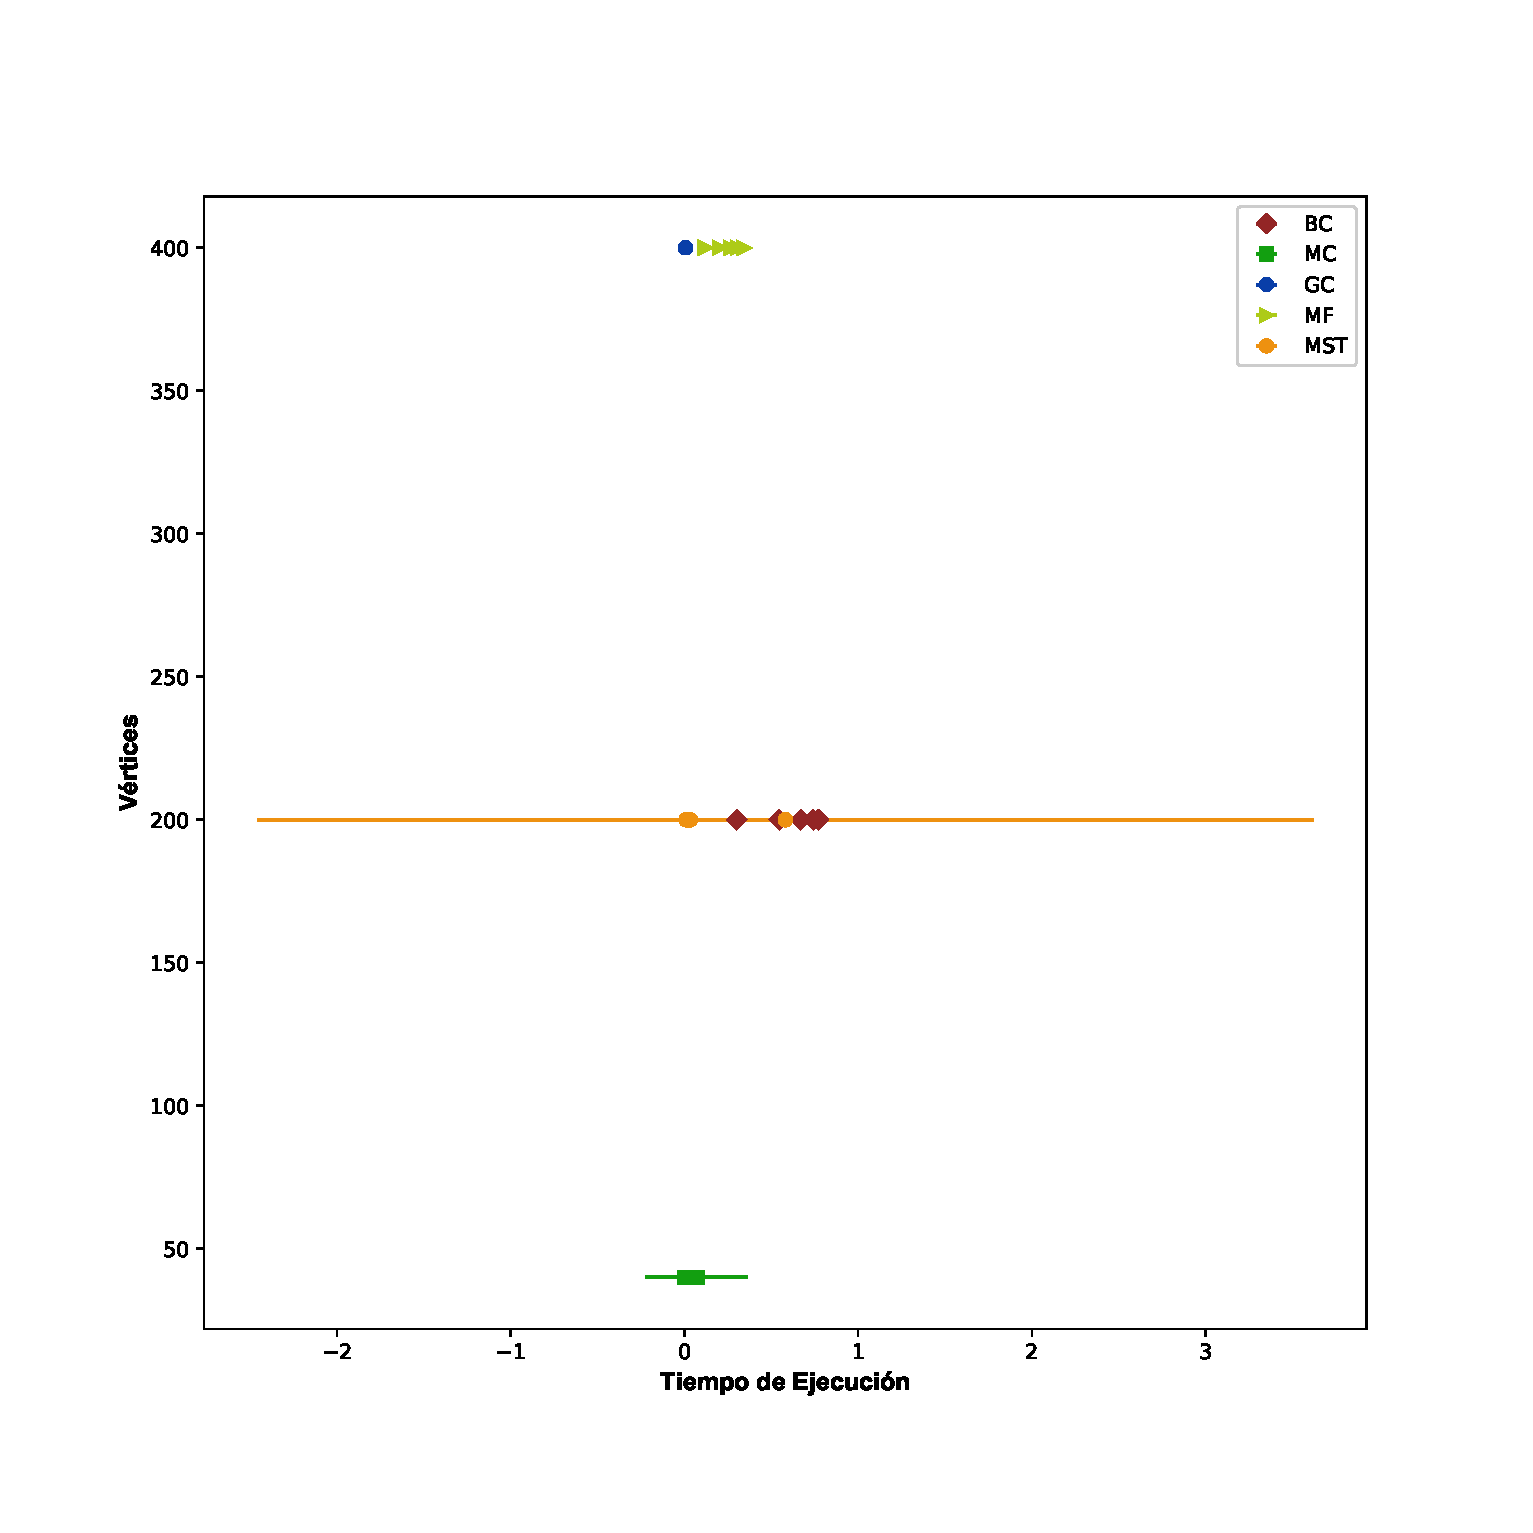
\includegraphics[scale=0.6]{Imagenes/Fig2.eps}
    \caption{Diagrama de disperción (cant. nodos vs media-algoritmo)}
    \label{fig:Fig2}
\end{figure}

En la figura \ref{fig:Fig3} de la página \pageref{fig:Fig3} se muestra la relación entre la media de cada algoritmo y la cantidad de arcos que se emplearon por grafo. En esta se aprecia que como tendencia general en los algoritmos medidos, al aumentar el número de arcos aumenta la media, el que más aumenta en su media es el algoritmo BC, en el algoritmo GC el valor de la media permanece casi constante a pesar del aumento de arcos, lo cual tiene sentido por el modo en que opera el mismo, el algoritmo MS actua de manera similar. Para el MC es casi despreciable la cantidad de arcos, debido a la demora del mismo se decidió disminuirlos.

Seguidamente se muestra el fragmento de código:

\lstinputlisting[language=Python, firstline=58, lastline=97]{Scatterplot.py}
\newpage
\begin{figure}[htbp]
    \centering
    \includegraphics[scale=0.6]{Imagenes/Fig3.eps}
    \caption{Diagrama de disperción (cant. arcos vs media-algoritmo)}
    \label{fig:Fig3}
\end{figure}
    
\newpage
\bibliography{Referencias_3}
\bibliographystyle{plainnat}
\end{document}